\documentclass[a4paper, twoside, 11pt, openright]{article}
\usepackage[utf8]{inputenc}
\usepackage{polski}
\usepackage{float}
\raggedbottom

\usepackage[left=3.0cm, right=2.0cm, top=2.5cm, bottom=2.5cm]{geometry}

% PERSONAL data about the thesis
\newcommand{\myTitle}{Metodyka porównania algorytmów prognozy do wspomagania decyzji giełdowych}
\newcommand{\myName}{Nikodem Wiśniewski}
\newcommand{\myNumber}{260907}
\newcommand{\myThesisType}{Praca dyplomowa magisterska}
\newcommand{\myCourse}{Informatyka}
\newcommand{\myProf}{dr hab. inż. Jerzy Balicki}
\newcommand{\myFaculty}{Wydział Matematyki i Nauk Informacyjnych}
\newcommand{\myUni}{Politechnika Warszawska}
\newcommand{\myLocation}{Warszawa}
\newcommand{\myYear}{2019}
\newcommand{\myKeywords}{}
\newcommand{\myKeywordsPL}{}


% BIBLIOGRAPHY
\usepackage{biblatex}
\usepackage{csquotes}
\DeclareQuoteStyle[quotes]{polish}
{\quotedblbase}
{\textquotedblright}
[0.05em]
{\quotesinglbase}
{\fixligatures\textquoteright}
\DeclareQuoteAlias[quotes]{polish}{polish}
\DeclareQuoteOption{polish}

% DOCUMENT settings


\usepackage{graphicx}
\usepackage{multirow}
\usepackage{indentfirst}
\usepackage{wrapfig}
\usepackage[font=footnotesize, % equivalent to 9 pt font
			labelfont=bf, 
			justification=justified, 
			singlelinecheck=false]{caption} 
%\usepackage[justification=centering]{subcaption} % two images side by side captions
\usepackage{tabularx, booktabs} % pretty LaTeX tables
\usepackage{siunitx} % units SI e.g. \SI{10}{\kilogram\per\meter\square}
\usepackage{mathtools} % amsmath, symbols such as brackets, arrows, equation numbering only for referrenced eqs.
%\usepackage[parfill]{parskip} % spacing between paragraphs instead of indent
%\parfillskip 0pt plus 0.75\textwidth % get rid of widows at the end of paragraphs
\frenchspacing % for "Polish" spaces after the sentence
\usepackage{polski} % Polish rules of hyphenation
\usepackage{dashrule} % for dotted lines in declarations page
\usepackage{emptypage} % removes headers on empty pages
\usepackage{fancyhdr} % header and footer settings
\usepackage{subfigure}

\pagestyle{fancy}
\fancyhf{}
\newcommand{\fncyfront}{%
	\fancyhead[RO]{}
	\fancyfoot[RO]{}
	\fancyhead[LE]{}
	\fancyfoot[LE]{}
	\fancyhead[RE,LO]{}
	\fancyfoot[C]{}
	\renewcommand{\headrulewidth}{0pt}}
\newcommand{\fncymain}{%
	\fancyhead[RO]{{\footnotesize \rightmark}}
	\fancyfoot[RO]{\thepage}
	\fancyhead[LE]{{\footnotesize \leftmark}}
	\fancyfoot[LE]{\thepage}
	\fancyfoot[C]{}
	\renewcommand{\headrulewidth}{0.3pt}}
	
\renewcommand*{\tablename}{Tabela} 
	
\newcolumntype{P}[1]{>{\centering\arraybackslash}p{#1}}
\newcolumntype{M}[1]{>{\centering\arraybackslash}m{#1}}



% FONT settings
\usepackage[T1]{fontenc}
\usepackage{uarial} % you can change to 'helvet' for Helvetica clone, 'uarial' for Arial clone, 'lmodern' for Latin Modern
%\renewcommand{\familydefault}{\sfdefault} % change font to sans serif
\usepackage{amsfonts} % mathematical fonts
\usepackage{inconsolata} % monospaced font in urls and \texttt
%\usepackage{url}
%\urlstyle{same}

% DEBUG
\usepackage{lipsum}
\usepackage{etoolbox} % removes page number in table of contents
\patchcmd{\chapter}{plain}{empty}{}{}


\begin{document}
\fncyfront
%*******************************************************
% Titlepage
%*******************************************************
\begin{titlepage}
\begingroup
\begin{center}		
			
\includegraphics[width=1.0\textwidth]{img/pw_header}
			
			\vspace{1.0cm}
			\fontsize{24}{30}\selectfont\myThesisType
			\fontsize{12}{14}\selectfont
			
			\vspace{0.5cm}
			na kierunku \myCourse \\
			\vspace{1cm}
			{\fontsize{14}{18}\selectfont \myTitle} \\ 
			
			\vspace{1.5cm}
			\fontsize{21}{25}\selectfont \myName \\
			\fontsize{12}{14}\selectfont
			Numer albumu \myNumber \\

			\vspace{6.5cm}
			promotor \\
			\myProf \\
			\vspace{0.5cm}
			\vfill 
			Warszawa, \myYear
        \vfill                      
\end{center}
\endgroup
\end{titlepage}

\newpage
\hfill
\begin{table}[b]
\centering
\begin{tabular}[t]{ccc}
............................................. & \hspace*{100pt} & .............................................\\
podpis promotora & \hspace*{100pt} & podpis autora
\end{tabular}
\end{table}

\fncymain

\newpage

\section{Opis pracy}

\subsection{Giełda}

\subsection{Hipoteza błądzenia losowego}

Zgodnie z hipotezą błądzenia losowego ceny akcji zmieniają się według losowych zmian ceny, a wyszukiwanie wzorców z przeszłości nie ma korzystnego wpływu na strategie inwestycyjne  \cite{randwalk}. 

\section{Predykcja}

Przewidywanie wartości akcji jest główną zagwostką zarówno inwestorów indywidualnych jak i instytucjonalnych. Skuteczne odgadywanie przyszłych wzrostów lub spadków pozwoliłoby na osiąganie ponadprzeciętnych zysków i unikanie strat.

\subsection{Dostępne dane}

Przed przystąpieniem do wyboru metod warto również zastanowić się nad danymi wejściowymi do algorytmu przewidującego. Podstawowymi danymi prezentowanymi na giełdzie są:
\begin{itemize}
\item{Data}
\item{Cena zamknięcia} cena akcji pod koniec dnia
\item{Cena otwarcia} cena akcji na początku dnia
\item{Ilość akcji w obrocie danego dnia}
\item{Najniższa cena akcji danego dnia}
\item{Najwyższa cena akcji danego dnia}
\end{itemize}

Wszystkie te dane mogą być wykorzystywane do przewidywania cen akcji.

 Przy korzystaniu z wartości cen akcji należy również uwzględnić tak zwane \textit{splity}. W momencie gdy jakaś spółka decyduje się na split oznacza to wówczas że każda z jej akcji dzieli się na dwie akcje o cenie wynoszącej połowe pierwotnej ceny za sztukę. Taki zabieg pozwala na zmniejszenie ceny pojedyńczej akcji dzięki czemu może stać się ona dostępna dla większej ilości inwestorów. 


\subsection{Parametr przewidywany}

Najbardziej pożytecznym parametrem akcji, którego przewidywanie daje inwestorowi największe szanse na zysk jest \textit{cena zamknięcia}. Do tematu prognozowania można podejść na dwa sposoby:
\begin{itemize}
\item{\textbf{dokładny}, przewidywanie konkretnych wartości akcji}
\item{\textbf{dyskretny}, predyckja wzrostu, spadku lub utrzymania ceny}
\end{itemize}

Korzystniejszym podejściem jest przewidywanie dokładnych cen akcji, gdyż pozwoli na lepsze wykorzystanie uzyskanej wiedzy. Druga metoda ze względu na ograniczenie dziedziny wyników daje szanse na dokładniejsze odwzorowanie wartości akcji w przyszłości.

\subsection{Metodyka i ocena metod}

Ponieważ zagadnienie przewidywania giełdy jest nietrywialne ze względu na losowe wahania wpływające na ceny akcji, do oceny każdej z metod predykcji zostaną wykorzystane zróżnicowane parametry:
	
\begin{itemize}
\item{\textbf{Prognozowanie dokładne/dyskretne} }
\item{\textbf{Liczba dni}, z których prognozowana jest wartość.}
\item{\textbf{Dobór danych pobranych z giełdy} - selekcja wartości wejściowych}

\end{itemize}

Ze względu na fakt, iż przy prognozowaniu na pare dni do przodu dochodzi do nałożenia się błędów predykcji. Na przykład jeżeli prognozowana jest wartość z dwóch dni historii na trzy dni do przodu, to wówczas trzeci prognozowany dzień będzie oparty na prognozach dwóch poprzednich dni. Z tego powodu przewidywać będziemy wartość ceny następnego dnia.



%Jakie spółki wybrać do porównania wyników? Najlepiej różnorodne, prezentujące małe/duże przedsiębiorstwa z różnych sektorów o różnych wariancjach ceny i niskiej korelacji. Warto porównać również różne okresy np. w momencie kryzysu 2008/9.


\subsection{Regresja liniowa}
%Po 1 wrzucic wykres z wnioskami.z predykcji regresja wartosci dokladnych
%Po 2 przekuć to na predykcje wzrostu spadku utrzymania cen i wykazac ze jest to slaba metoda
%Ad 1 zrobic metode ktora rysuje caly wkyres tylko dla 1 miesoaca

Jedną z naiwnych metod przewidywania wartości funkcji jest regresja liniowa. Pierwszą próbą dla tego modelu było przewidzenie ceny zamknięcia z kolejnego dnia przy posiadaniu danych z dnia poprzedniego.

\begin{figure}[H]%
\centering
\subfigure[Wykres rzeczywistych wartości]{%
\label{l_r_stock_data}
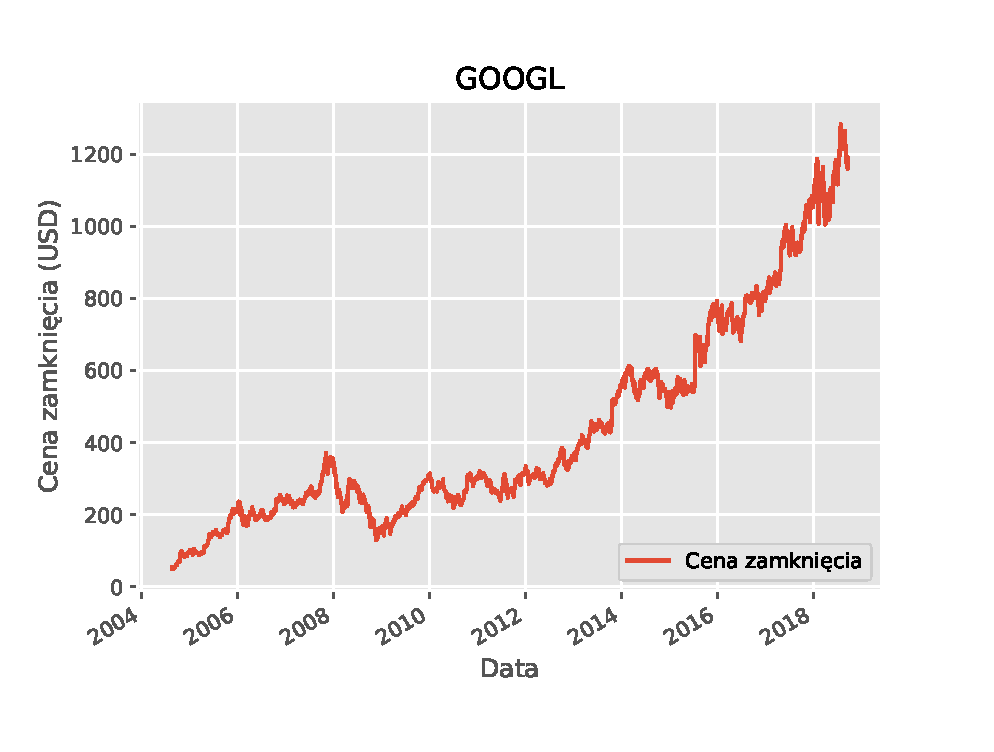
\includegraphics[scale=0.46]{img/linear_regression/l_r_stock_data}}%
\qquad
\subfigure[Wkyres rzeczywistych oraz przewidywanych wartości]{%
\label{l_r_1_day_full}
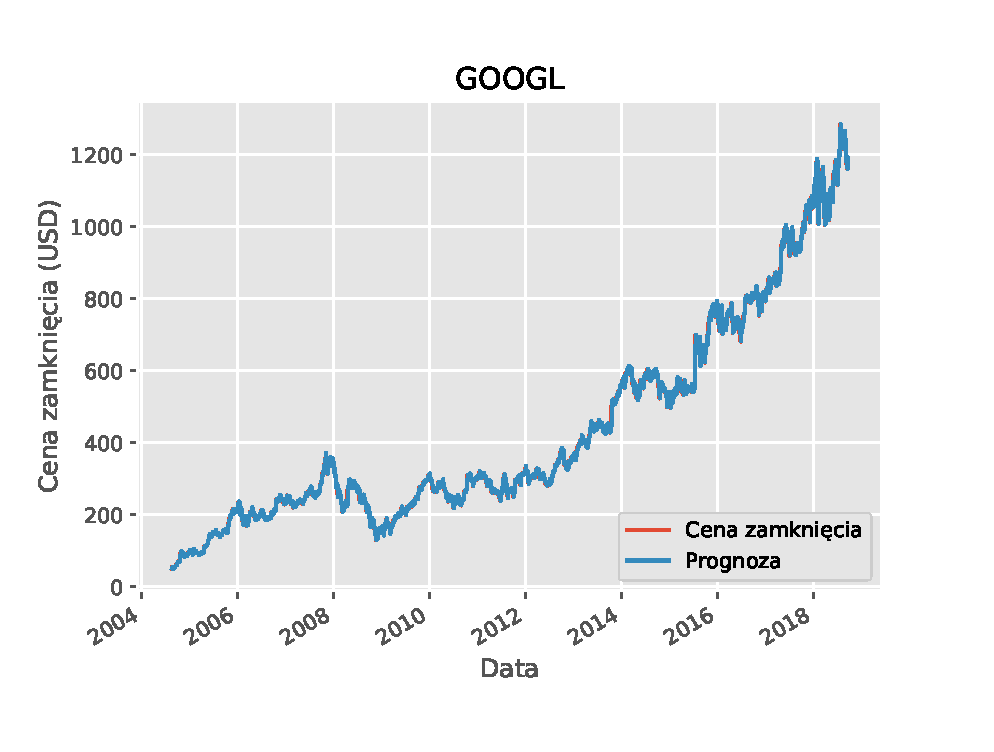
\includegraphics[scale=0.46]{img/linear_regression/l_r_1_day_full}}%
\caption{Wykres dla spółki \textit{GOOGL}}
\label{linear_regression_1}
\end{figure}

Z rysunku \ref{linear_regression_1} wynika iż prognozowane wartości pokrywają się z rzeczywistymi. Po obliczeniu błędu model daje nam dokładność na poziomie około  $99,934\%$. Wydaje się to być doskonałym wynikiem. Aby upewnić się o wartości modelu należy przyjrzeć się wykresowi z bliska.

\begin{figure}[H]
\centering 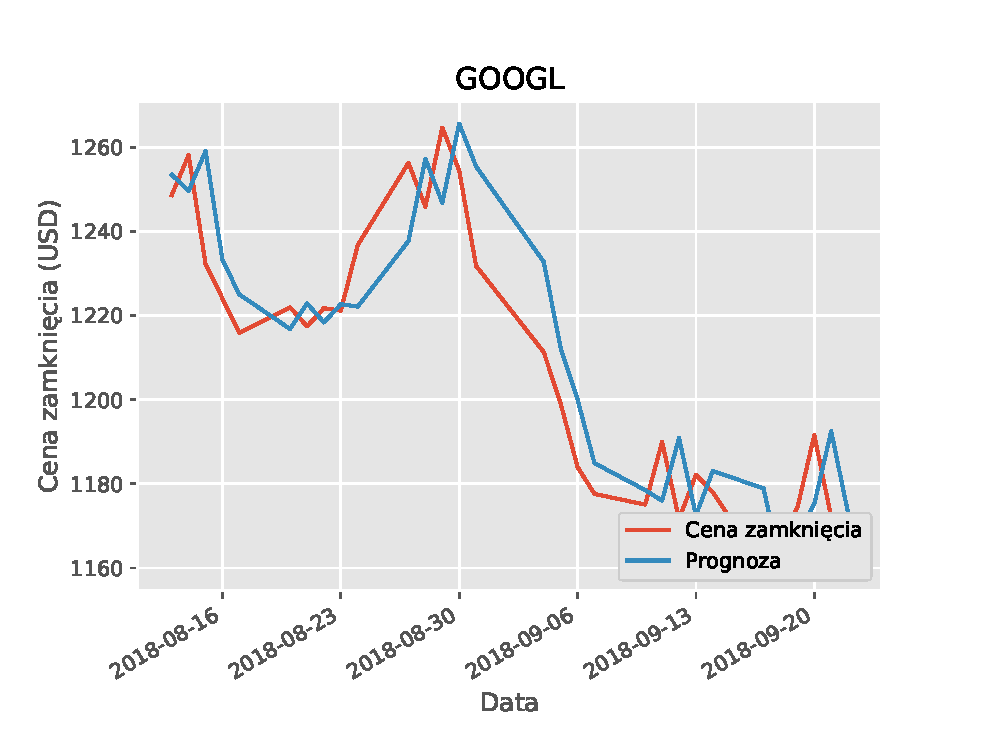
\includegraphics[scale=0.9]{img/linear_regression/l_r_1_day_last_30}
\caption{Wykres dla spólki \textit{GOOGL} z ostatnich 30 dni}
\label{l_r_1_day_last_30}
\end{figure}

Na rysunku \ref{l_r_1_day_last_30} widać że prognozowane wartości są w rzeczywistości delikatnie zniekształconym obrazem przeszłych notowań spółki. Dokładność na poziomie $~99\%$ została osiągnięta ze względu na małe wahania w cenie. Logicznie rzecz biorąc nie jest to dobra metoda przewidywania przyszłości. Gdy cena jest w lokalnym maksimum wówczas inwestor powinien sprzedać posiadane akcje, jednak model przewiduje dalsze wzrosty ceny i wprowadza inwestora w błąd. Analogiczna sytuacja dzieje się przy minimach lokalnych ceny akcji.

\bigskip

W celu skutecznej oceny modelu, który ma służyć do celów inwestycyjnych, zamiast przewidywania dokładnej ceny zamknięcia należy przewidywać wzrosty oraz spadki ceny. Binarne przewidywanie z dnia na dzień może jednak okazać się nieprzydatne ze względu na to jak przebiega obrót akcjami. Akcje kupuje i sprzedaje się za pomocą domu maklerskiego, który pobiera prowizje za każdą transakcję. Obecnie najniższe prowizje na polskim rynku są na poziomie $0,19\%$ za transakcje. Pojedyńcza operacja dająca zarobić na przewidzianej cenie wymaga kupienia, a następnie sprzedania akcji, wobec czego łączna prowizja wyniesie przy zaokrągleniu $0,4\%$. Wszystkie wahania cen poniżej tej wartości są teoretycznie bez znaczenia dla inwestora. W związku z powyższym wnioskowaniem należy zastosować model, który przewiduje trzy wartości:
\begin{itemize}
\item spadek ceny poniżej $0,4\%$
\item wzrost ceny powyżej $0,4\%$
\item utrzymanie zmiany ceny w przedziale $(-0,4, 0.4)\%$
\end{itemize}



\newpage

\renewcommand{\refname}{Bibliografia}
\begin{thebibliography}{9}

\bibitem{randwalk}
  Burton G. Malkiel,
  \textit{Random Walk Down Wall Street: The Time-Tested Strategy for Successful Investing}.
  W. W. Norton Company,
  2007.

\end{thebibliography}

\end{document}